\documentclass[11pt,a4paper]{article}
\usepackage[utf8]{inputenc}
\usepackage[T1]{fontenc}
\usepackage[spanish]{babel}
\usepackage[margin=2.5cm]{geometry}
\usepackage{graphicx}
\usepackage{hyperref}
\usepackage{booktabs}
\usepackage{enumitem}
\usepackage[numbers]{natbib}

\graphicspath{{resultados/figures/}}
\hypersetup{colorlinks=true,linkcolor=blue,citecolor=blue,urlcolor=blue}

\title{Framework IA para análisis de datos\\\large Informe técnico y resultados reproducibles}
\author{Laboratorio de análisis de datos}
\date{Noviembre de 2026}

\begin{document}
\maketitle
\begin{abstract}
Se presenta una aplicación local para explorar y preparar conjuntos de datos y ejecutar análisis de agrupamiento,
clasificación y regresión. El sistema integra una interfaz Streamlit, un controlador, servicios reutilizables y un
sistema multiagente con coordinador, registro, fábrica, mensajería y agentes especializados. Se describen la
arquitectura, el ciclo de una solicitud, la extensión dinámica y la trazabilidad, además de tres experimentos
reproducibles de aprendizaje automático. Los resultados se generan con el mismo backend que utiliza la aplicación.
\end{abstract}
\tableofcontents
\newpage

\section{Objetivo y arquitectura}
El objetivo es ofrecer una interfaz local para cargar datos, explorar variables, preparar información y ejecutar
algoritmos de aprendizaje automático. El dashboard de Streamlit utiliza \texttt{FrameworkController} como entrada
única al backend. El controlador valida solicitudes, coordina servicios y agentes, y registra cada ejecución.

El proyecto se organiza en capas; la interfaz se construye con Streamlit \citep{streamlitdocs}:
\begin{itemize}[nosep]
  \item \texttt{frontend/}: navegación, páginas y componentes de Streamlit.
  \item \texttt{framework\_ia/controller.py}: coordinación entre interfaz y backend.
  \item \texttt{framework\_ia/services/}: carga, transformación y registro de ejecuciones.
  \item \texttt{framework\_ia/ml/}: EDA, preprocesamiento y algoritmos de aprendizaje.
  \item \texttt{framework\_ia/agents/}: agencia, coordinador, registro, fábrica, bus y agentes especializados.
  \item \texttt{framework\_ia/persistence/}: almacenamiento local de experimentos y configuración.
\end{itemize}
Los algoritmos y transformaciones se implementan con bibliotecas científicas de Python \citep{pedregosa2011scikit}.
Para los experimentos de este informe se desactivó el servicio externo de IA; por tanto, no se requieren claves ni
conexión a un proveedor para reproducir los resultados.

\begin{figure}[htbp]
  \centering
  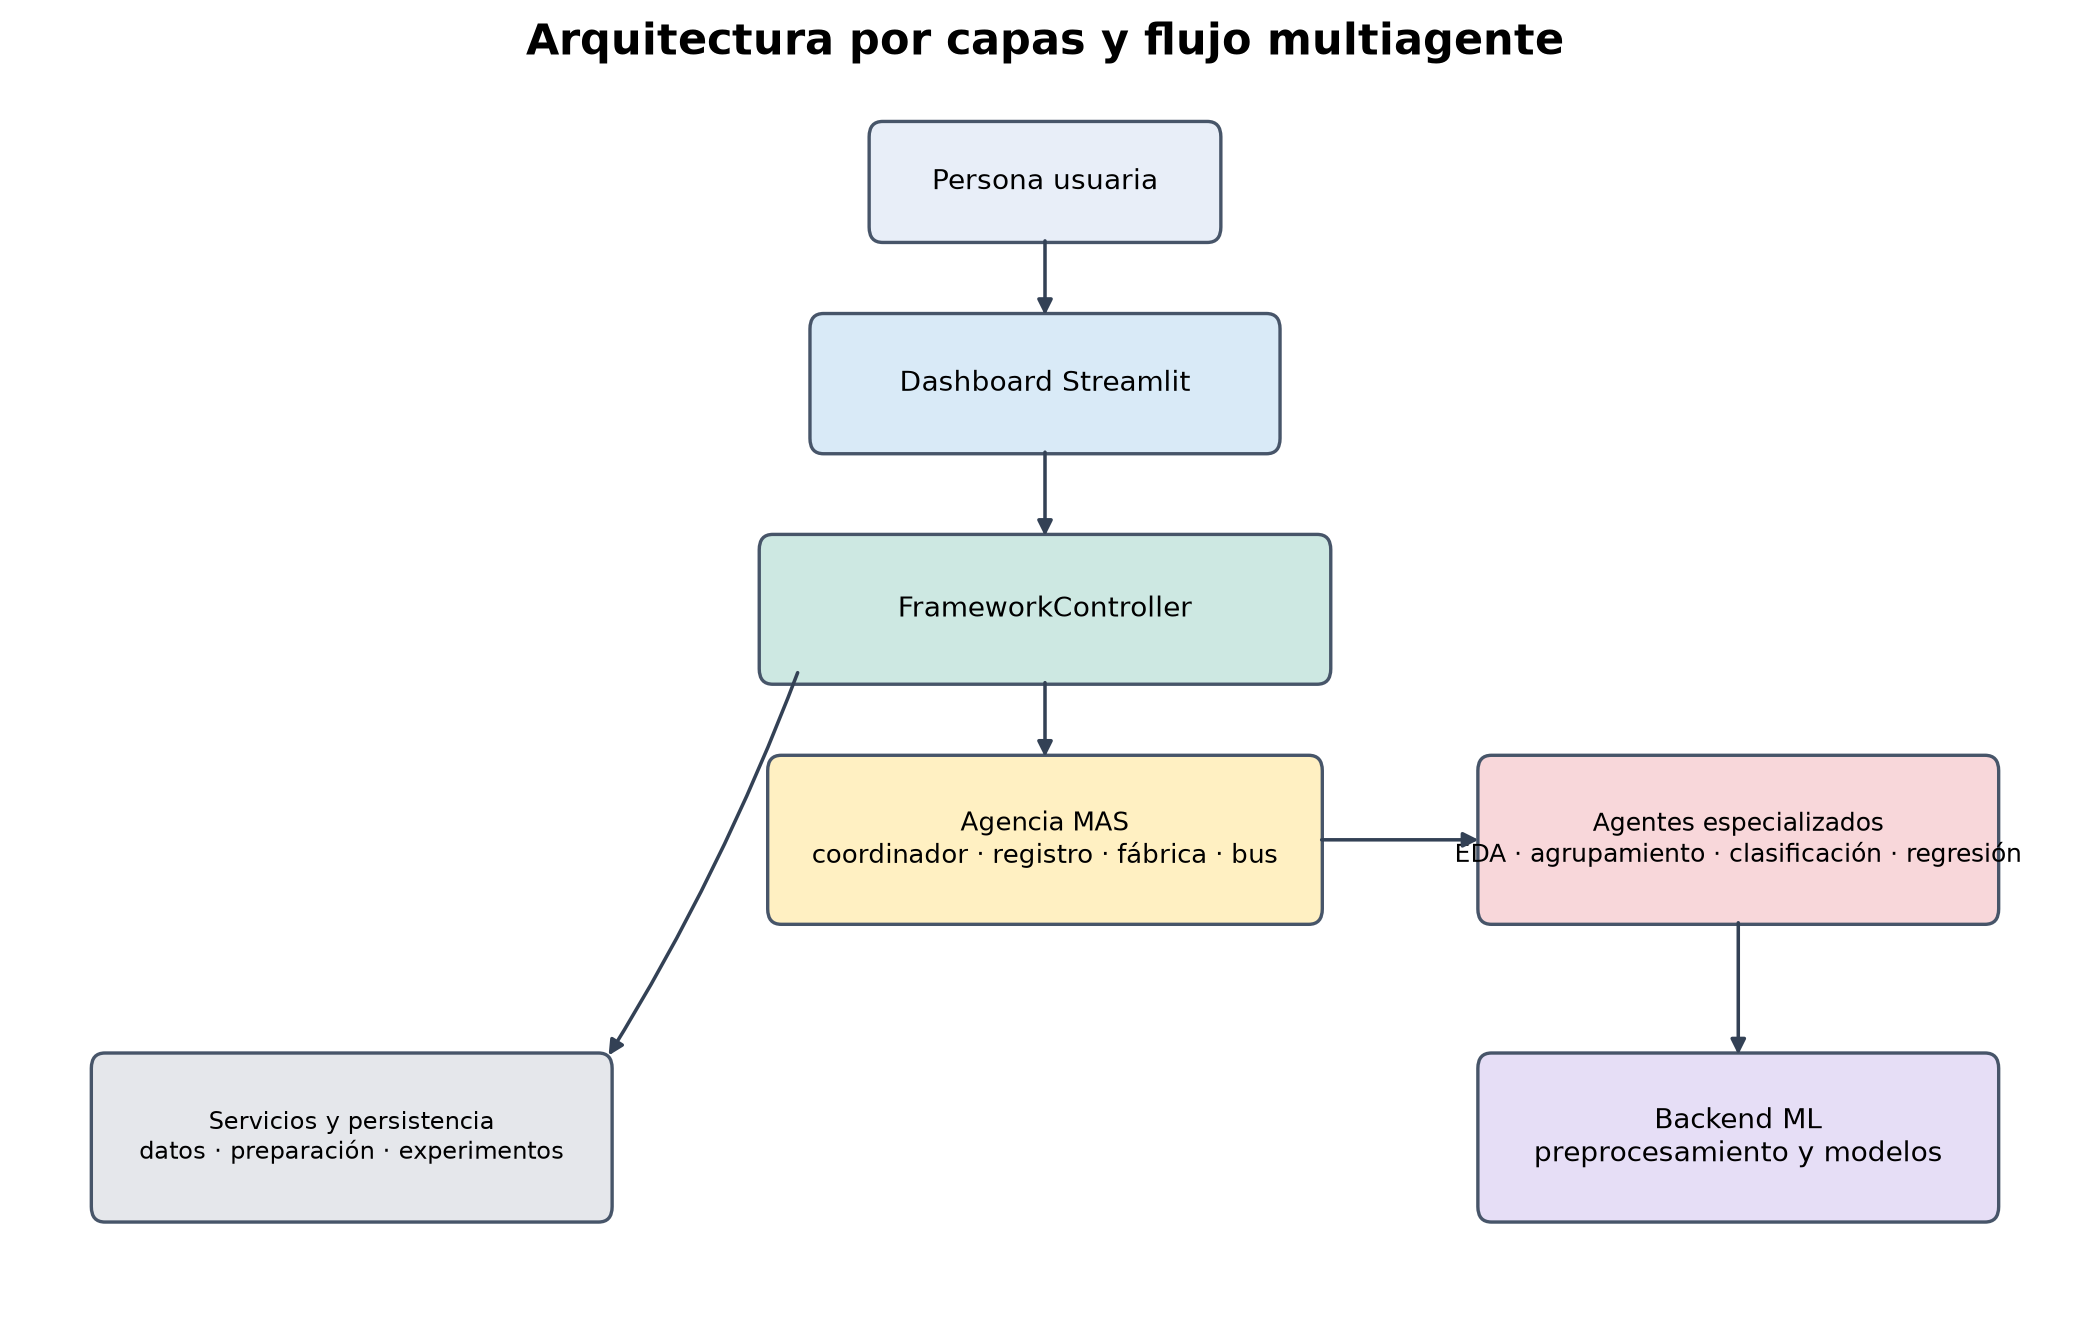
\includegraphics[width=\textwidth,height=0.72\textheight,keepaspectratio]{05_arquitectura_mas.png}
  \caption{Capas de la aplicación y recorrido de una solicitud desde Streamlit hasta los agentes y el backend ML.}
  \label{fig:arquitectura-mas}
\end{figure}

\section{Diseño e implementación del sistema multiagente}
La arquitectura sigue el enfoque de agentes autónomos que cooperan mediante mensajes y servicios especializados;
la teoría de agentes distingue sus propiedades, arquitecturas y formas de interacción \citep{wooldridge1995agents}.
En esta implementación, cada agente expone una identidad, un estado y un conjunto de capacidades. El coordinador
resuelve la capacidad requerida a partir de la tarea, consulta el registro y delega sin depender de las clases
concretas de los agentes.

\subsection{Roles y capacidades}
\begin{center}
\small
\begin{tabular}{p{0.20\textwidth}p{0.31\textwidth}p{0.39\textwidth}}
\toprule
Componente & Responsabilidad & Capacidades principales \\
\midrule
Coordinador & Analiza solicitudes, descubre candidatos, delega y consolida resultados. &
\texttt{coordination.route} \\
Agente EDA & Perfila, resume, limpia y prepara los datos. &
\texttt{eda.profile}, \texttt{eda.summary}, \texttt{eda.clean}, \texttt{eda.preprocess} \\
Agente de agrupamiento & Ejecuta reducción dimensional, clustering y benchmarks. &
\texttt{clustering.pca}, \texttt{clustering.kmeans}, \texttt{clustering.hac}, \texttt{clustering.benchmark} \\
Agente de clasificación & Entrena clasificadores y compara configuraciones. &
\texttt{classification.train}, \texttt{classification.benchmark}, \texttt{classification.auto} \\
Agente de regresión & Entrena regresores y compara configuraciones. &
\texttt{regression.train}, \texttt{regression.benchmark}, \texttt{regression.auto} \\
\bottomrule
\end{tabular}
\end{center}

\subsection{Mensajería, coordinación y manejo de fallos}
Las solicitudes usan mensajes estructurados con emisor, receptor, tarea, performativa, contenido y un identificador
de correlación. El bus entrega y registra las solicitudes y respuestas; el identificador permite relacionar los
mensajes de una misma ejecución. El flujo de la Figura~\ref{fig:secuencia-mas} muestra cómo se conserva esta
trazabilidad hasta la presentación del resultado.

La agencia aplica una política \texttt{priority} para asignar la tarea al candidato mejor clasificado y probar otro
si el primero falla. Con \texttt{fanout}, todos los candidatos disponibles ejecutan la misma capacidad y el
coordinador compara sus métricas principales para escoger una respuesta. La ejecución es síncrona. Los agentes
mantienen estado de ciclo de vida y estadísticas de tareas; los experimentos guardan los agentes, decisiones,
métricas y mensajes de cada solicitud. Los errores de validación se devuelven al usuario y los fallos de ejecución
pueden provocar reintentos, fallback y degradación del estado del agente.

\subsection{Extensibilidad e integración}
La fábrica crea agentes desde tipos registrados y descubre plugins en
\texttt{framework\_ia/agents/plugins/}. Un plugin publica sus capacidades y se incorpora al registro y al bus;
el coordinador puede encontrarlo mediante la capacidad solicitada sin modificar su lógica central.
\texttt{docs/evidencias/dynamic\_agent\_log.md} registra una prueba con \texttt{knn\_auto}: el agente se crea en
ejecución y es seleccionado para \texttt{classification.train}. Las pruebas de integración ejercitan el recorrido
controlador--coordinador--agente--modelo y verifican el almacenamiento del resultado; una prueba de interfaz
comprueba la creación y prueba guiada desde el panel MAS.

\begin{figure}[htbp]
  \centering
  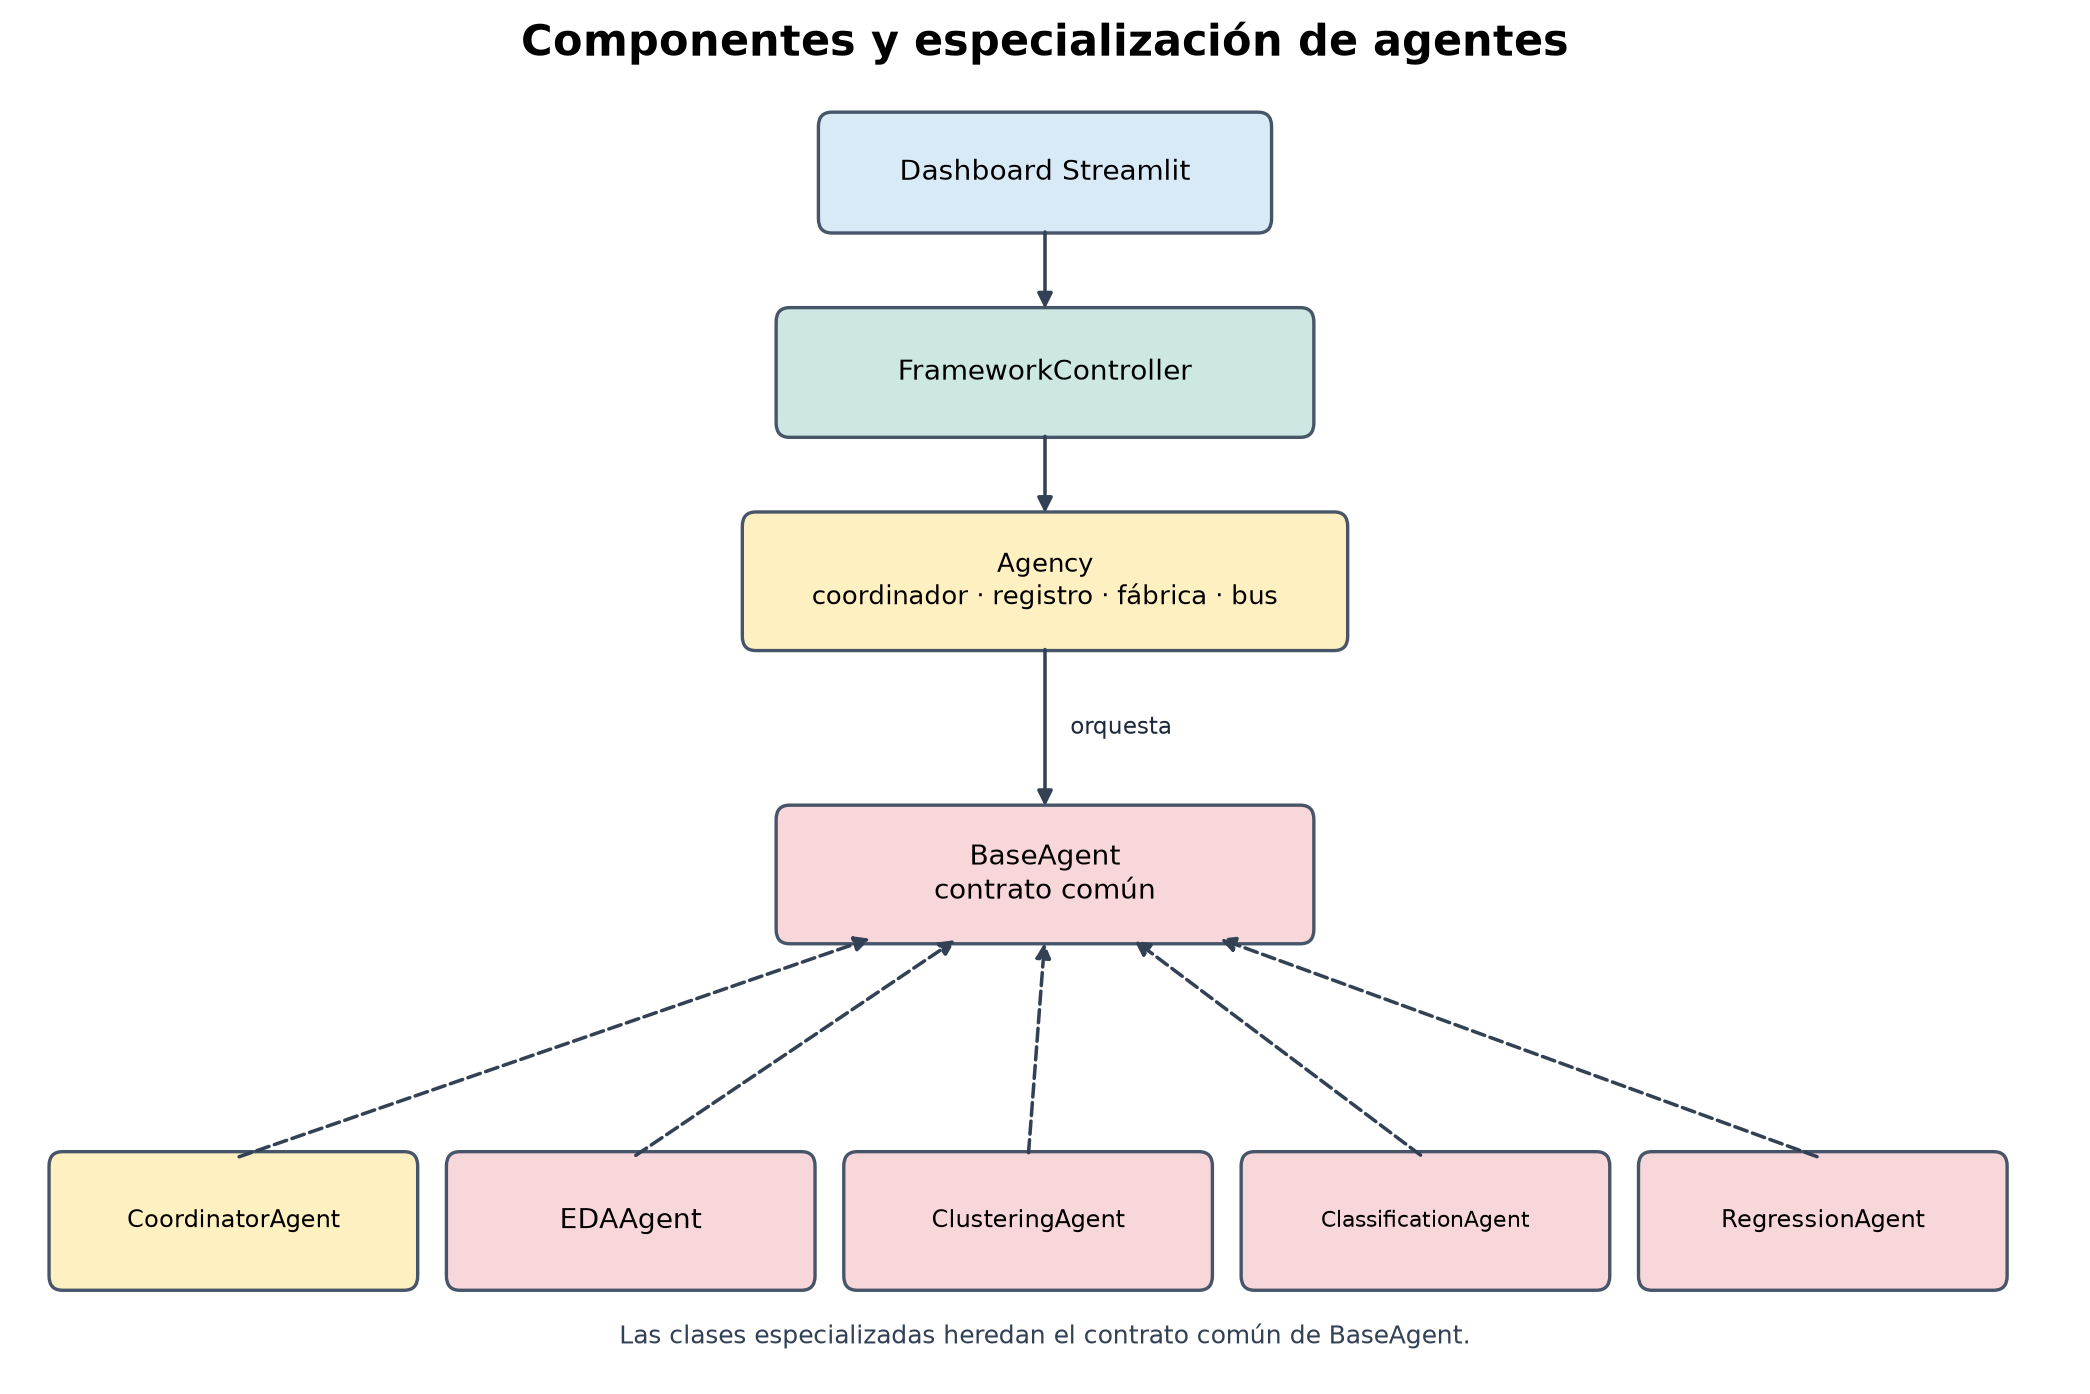
\includegraphics[width=\textwidth,height=0.72\textheight,keepaspectratio]{06_componentes_mas.png}
  \caption{Relación entre la agencia, el contrato común \texttt{BaseAgent} y los agentes especializados.}
  \label{fig:componentes-mas}
\end{figure}

\begin{figure}[htbp]
  \centering
  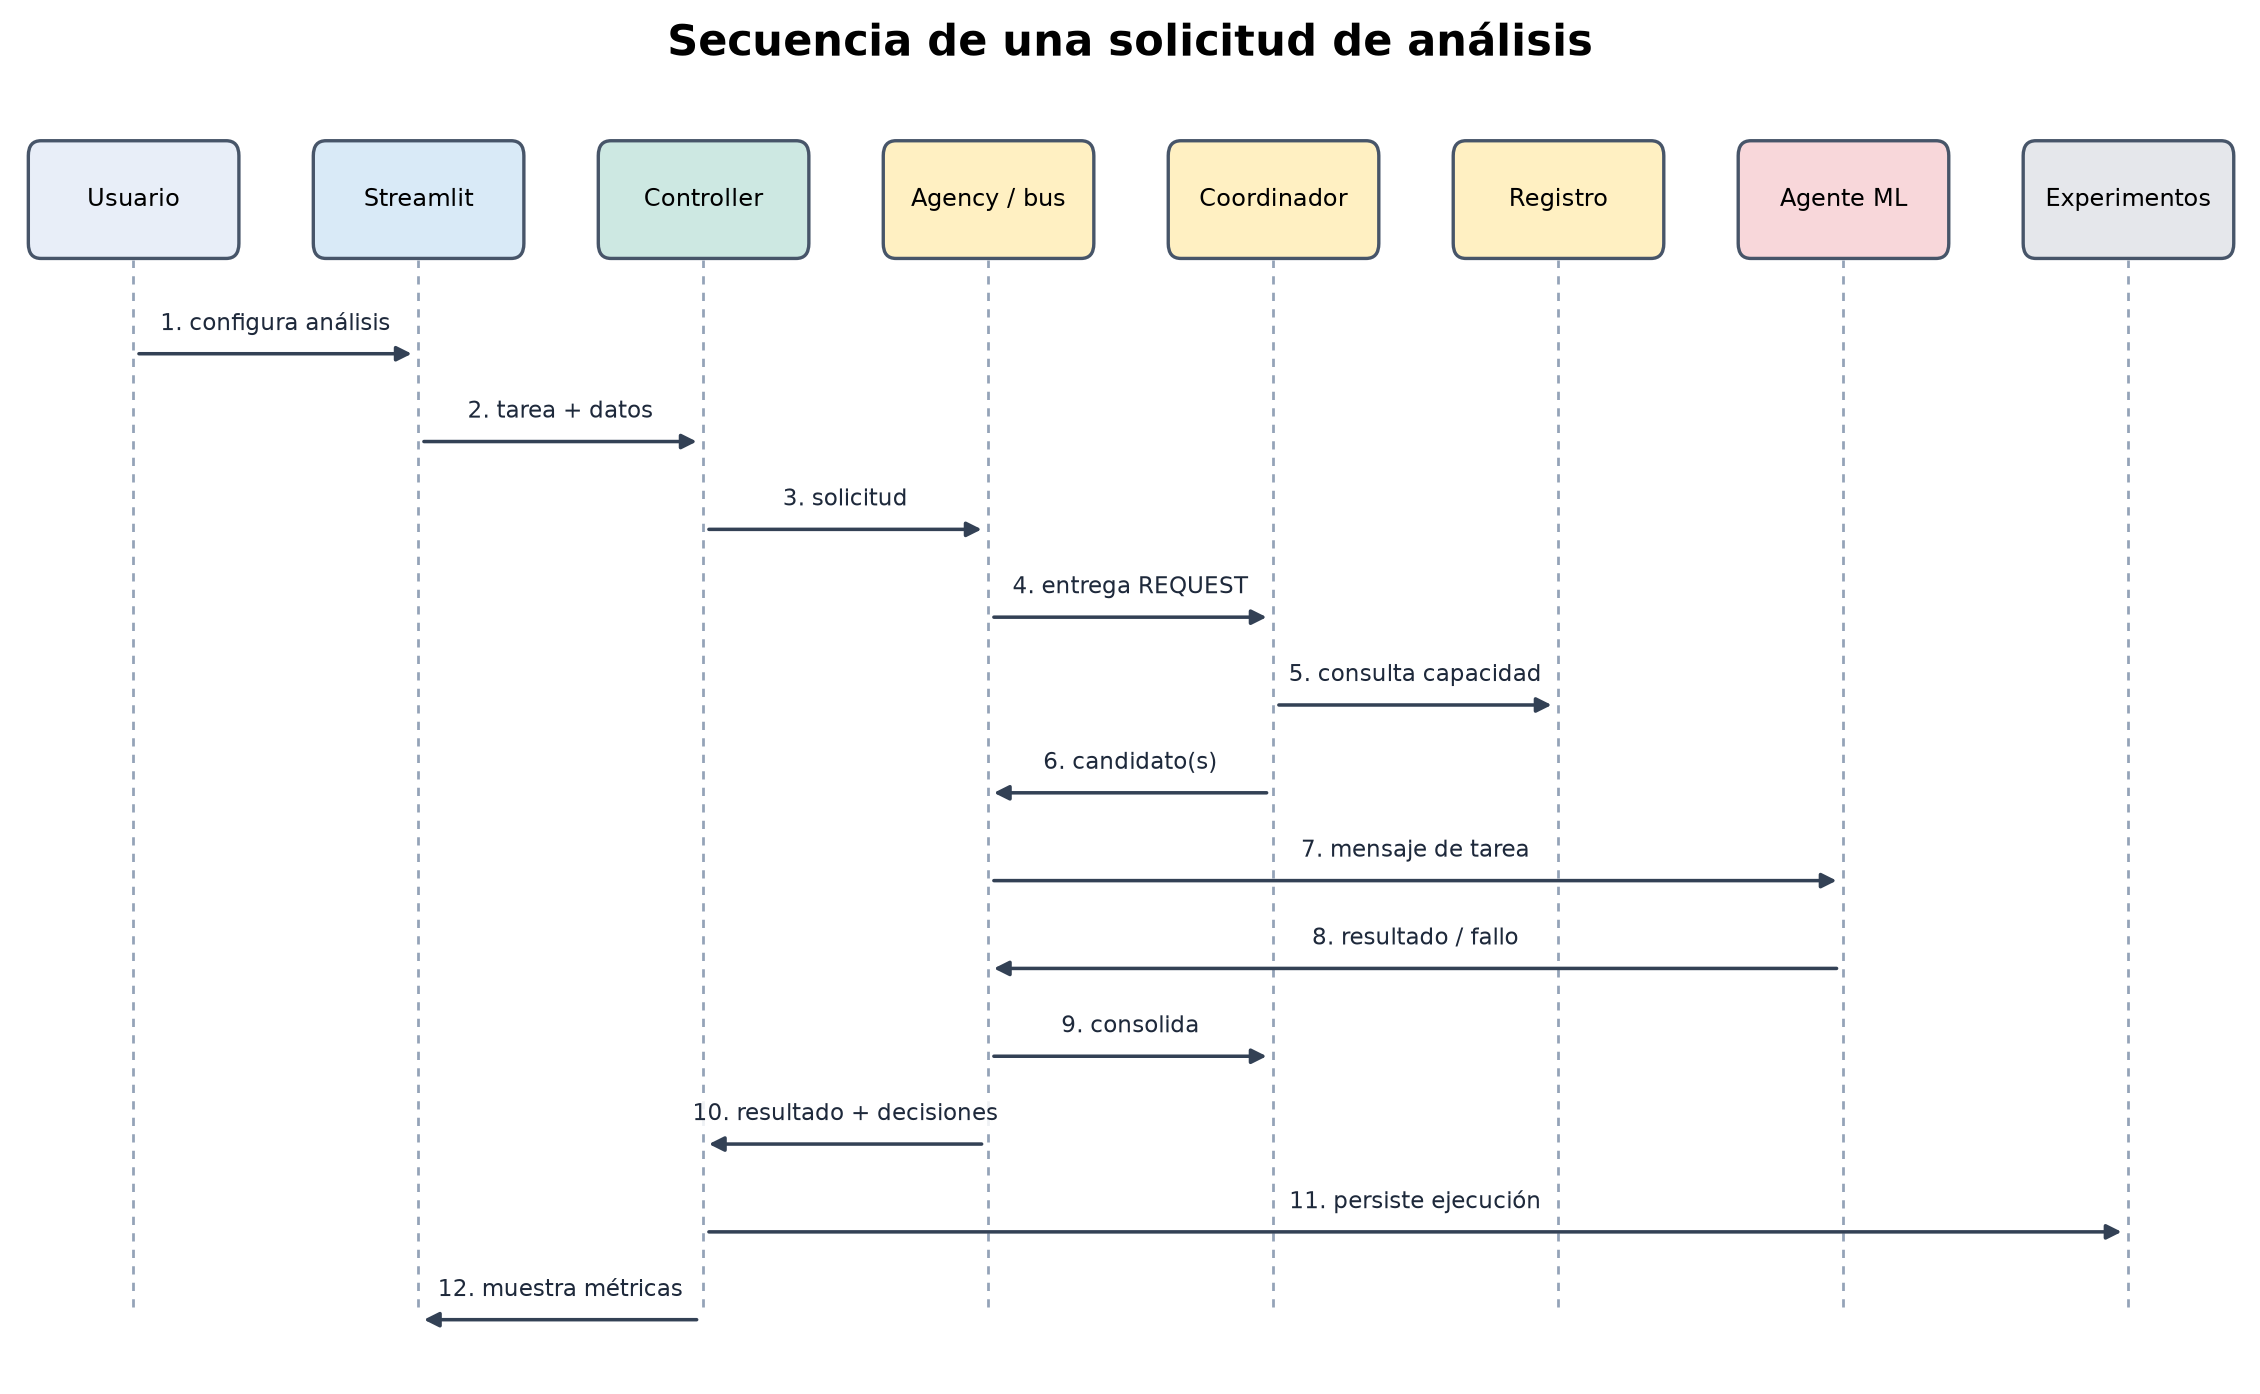
\includegraphics[width=\textwidth,height=0.72\textheight,keepaspectratio]{07_secuencia_mas.png}
  \caption{Secuencia de una tarea: enrutamiento, selección por capacidad, ejecución, persistencia y respuesta.}
  \label{fig:secuencia-mas}
\end{figure}

\section{Datos y diseño experimental}
\subsection{Clasificación}
Se utiliza \texttt{data/drug200.csv} (200 filas), con \texttt{Drug} como etiqueta y el catálogo de clasificadores
del proyecto para comparar configuraciones. El benchmark conserva la misma partición estratificada de 75\,\% para
entrenamiento y 25\,\% para prueba, con semilla 42. Para observar la variación por partición se evalúa además un
Random Forest de 200 árboles con las semillas 42, 43 y 44. La matriz de confusión del informe corresponde a la
semilla 42.

\subsection{Regresión}
Se utiliza \texttt{data/regression\_sample.csv} (300 filas), generado mediante
\texttt{scripts/generate\_regression\_sample.py}. El objetivo, \texttt{ingreso\_anual}, se construye a partir de
experiencia, nivel educativo, horas semanales, proyectos y departamento, más ruido aleatorio. No representa
ingresos observados ni personas reales. Se comparan las configuraciones del catálogo con una partición de 75/25 y
semilla 42. RidgeCV se evalúa adicionalmente con cinco valores de regularización y las semillas 42, 43 y 44.

\subsection{Agrupamiento}
Se utiliza \texttt{data/Mall\_Customers.csv} (200 filas), y se limitan las variables de entrada a
\texttt{Annual Income} (ingreso anual, k\$) y \texttt{Spending Score} (puntuación de gasto, 1--100) para no usar
identificadores ni atributos ajenos a la segmentación elegida. Las variables se estandarizan antes de aplicar
K-Means \citep{macqueen1967some} y HAC. Se comparan K-Means con $k=2,3,4$, HAC con enlace Ward y dos
configuraciones de PCA. El coeficiente silhouette se interpreta como una
medida de cohesión y separación entre grupos \citep{rousseeuw1987silhouettes}. La figura de segmentos muestra
K-Means con $k=3$ y una proyección a componentes principales.

\subsection{Reproducibilidad}
El script \texttt{scripts/run\_experiments.py} fija las semillas, desactiva el servicio de IA, crea las ejecuciones
en una carpeta temporal y genera las tablas CSV, el manifiesto JSON, la tabla LaTeX y las figuras. Los benchmarks
supervisados comparan configuraciones sobre una misma partición; sus resultados son comparables dentro de cada
tarea, no entre conjuntos distintos. La ejecución multi-semilla se reporta aparte para hacer explícita la
variabilidad observada.

\section{Resultados}
La tabla se genera directamente desde la salida del script, por lo que sus valores corresponden a los CSV y al
manifiesto distribuidos con este informe.
\begin{center}
\begin{tabular}{llr}
\toprule
Tarea y configuración & Resultado principal & Valor \\
\midrule
Benchmark de clasificación & Árbol (estándar) (F1 macro) & 0.9877 \\
Random Forest, 3 semillas & Exactitud media & 0.9867 \\
Random Forest, 3 semillas & F1 macro medio & 0.9918 \\
Benchmark de regresión & Regresión lineal múltiple (estándar) (RMSE) & 4512.96 \\
RidgeCV, 3 semillas & RMSE medio & 5038.24 \\
RidgeCV, 3 semillas & $R^2$ medio & 0.9445 \\
Benchmark de agrupamiento & K-Means k=4 (silhouette) & 0.4939 \\
\bottomrule
\end{tabular}

\end{center}

\begin{figure}[htbp]
  \centering
  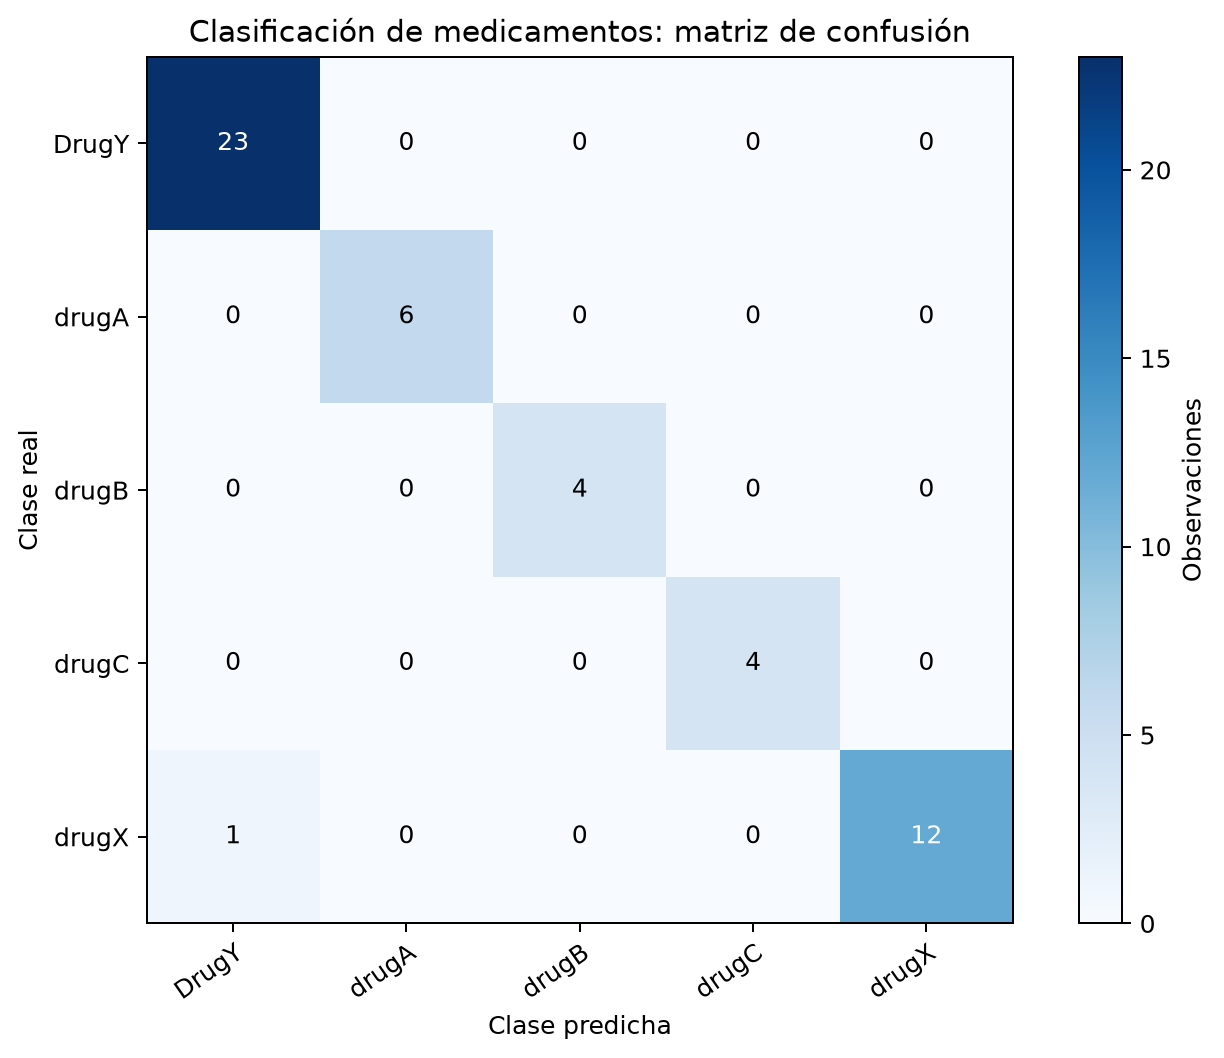
\includegraphics[width=0.82\textwidth]{01_matriz_confusion.png}
  \caption{Matriz de confusión para la clasificación con Random Forest en la partición de prueba de semilla 42.}
  \label{fig:confusion}
\end{figure}

\begin{figure}[htbp]
  \centering
  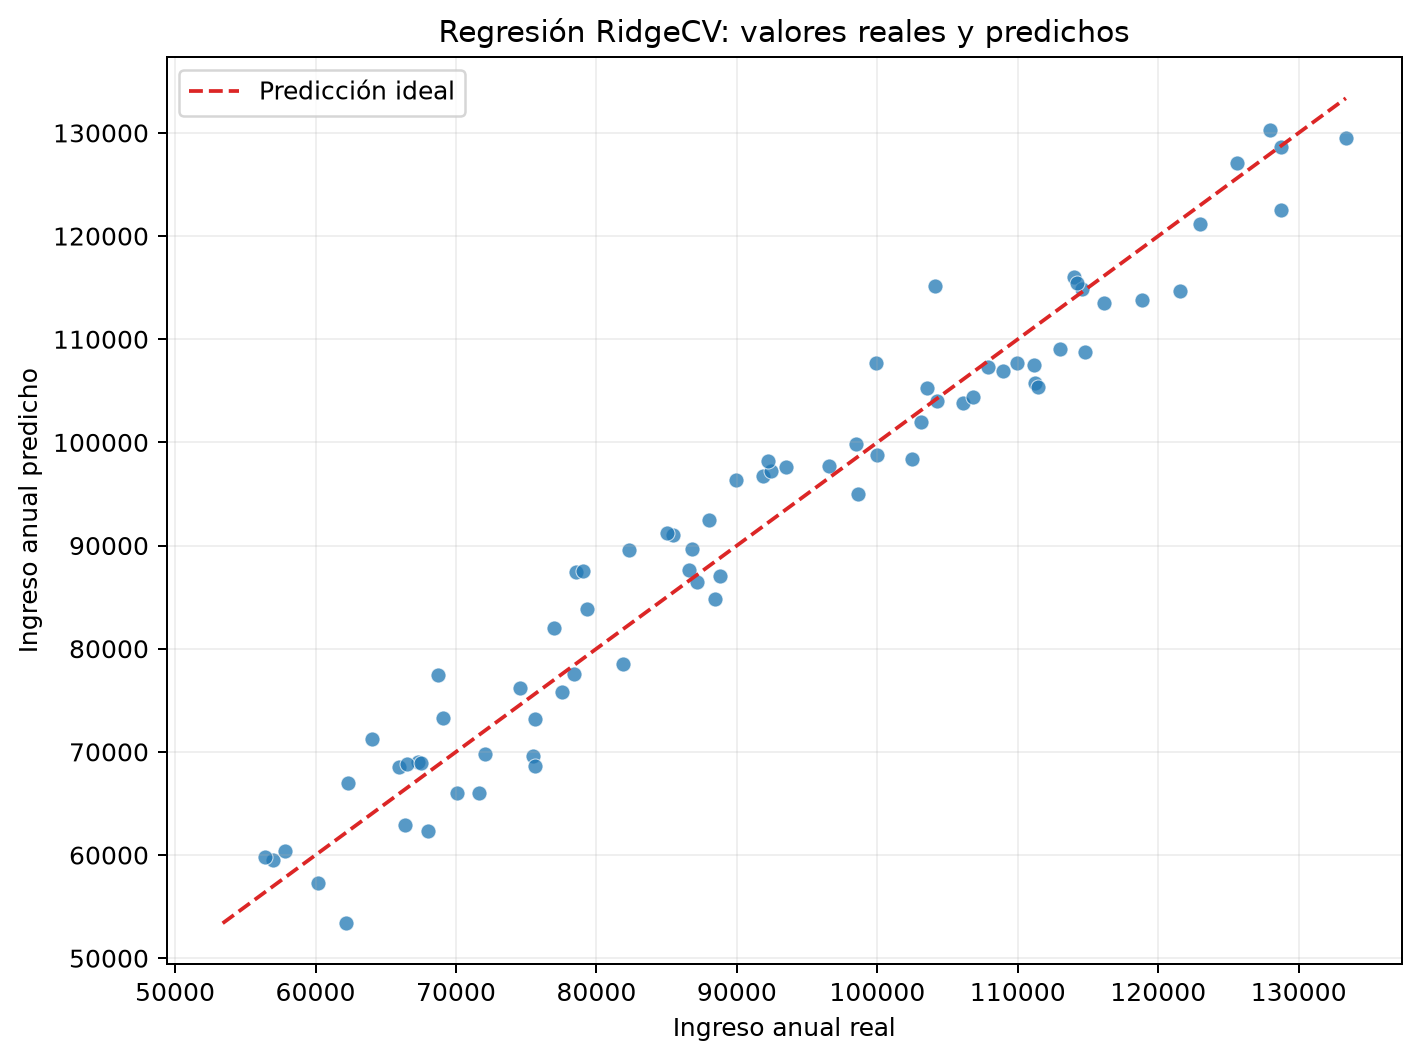
\includegraphics[width=0.82\textwidth]{02_regresion_real_predicho.png}
  \caption{Ingresos reales y predichos por RidgeCV para la partición de prueba de semilla 42. La diagonal indica
  predicción perfecta.}
  \label{fig:regresion}
\end{figure}

\begin{figure}[htbp]
  \centering
  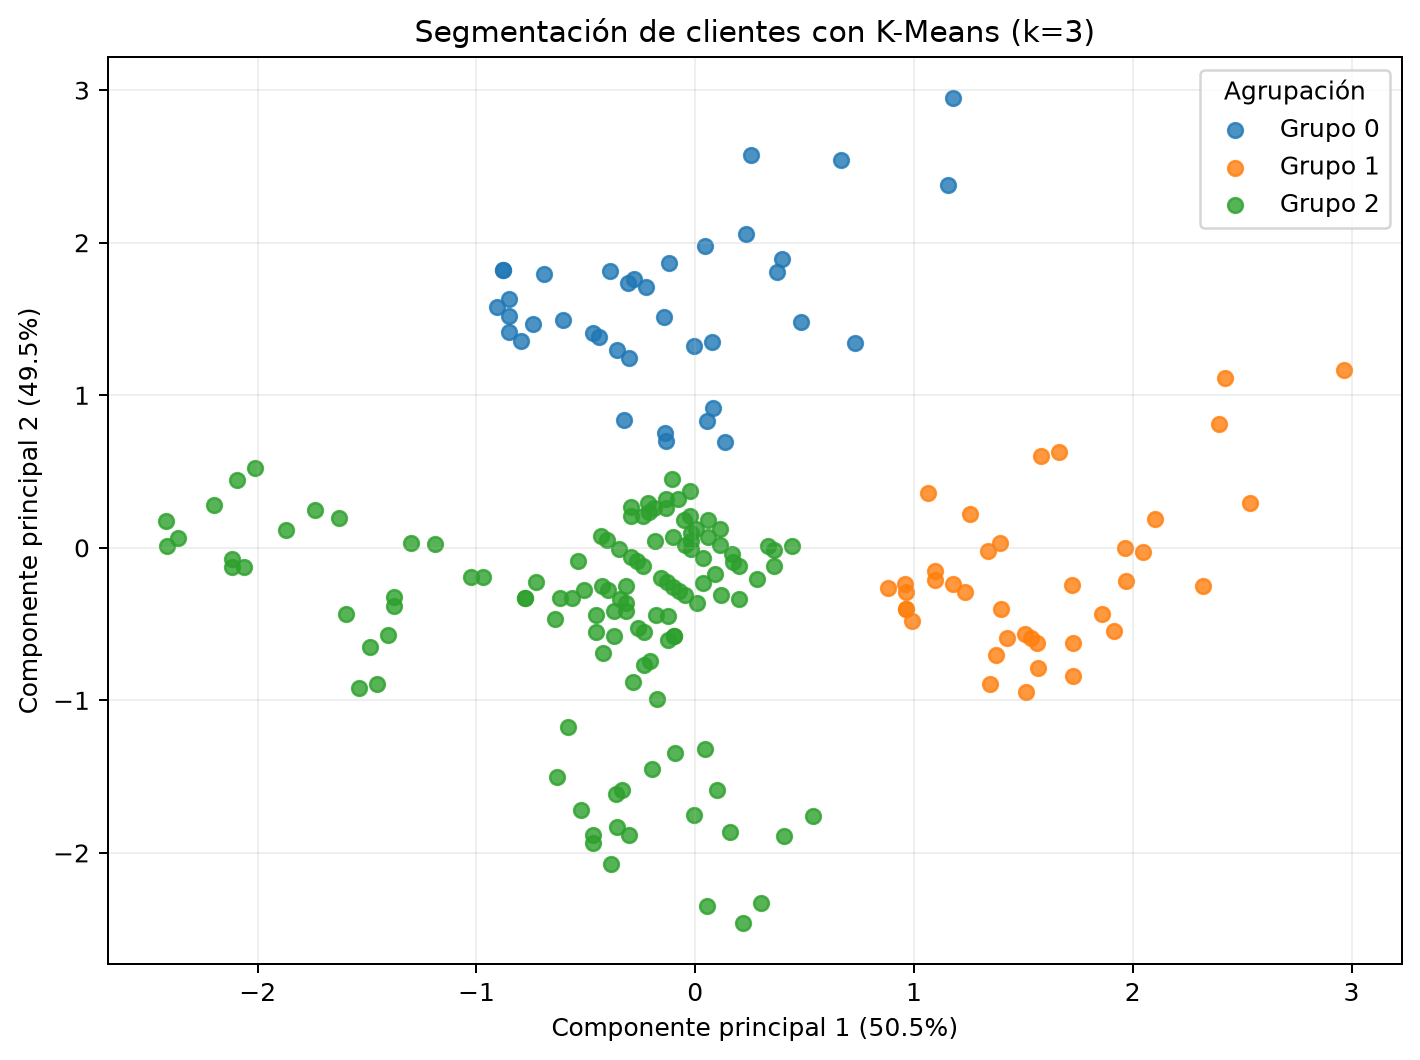
\includegraphics[width=0.82\textwidth]{03_segmentacion_clientes.png}
  \caption{Segmentación K-Means con $k=3$ sobre las dos variables seleccionadas, proyectada en componentes
  principales. El porcentaje de cada eje indica la varianza explicada por esa componente.}
  \label{fig:clusters}
\end{figure}

\begin{figure}[htbp]
  \centering
  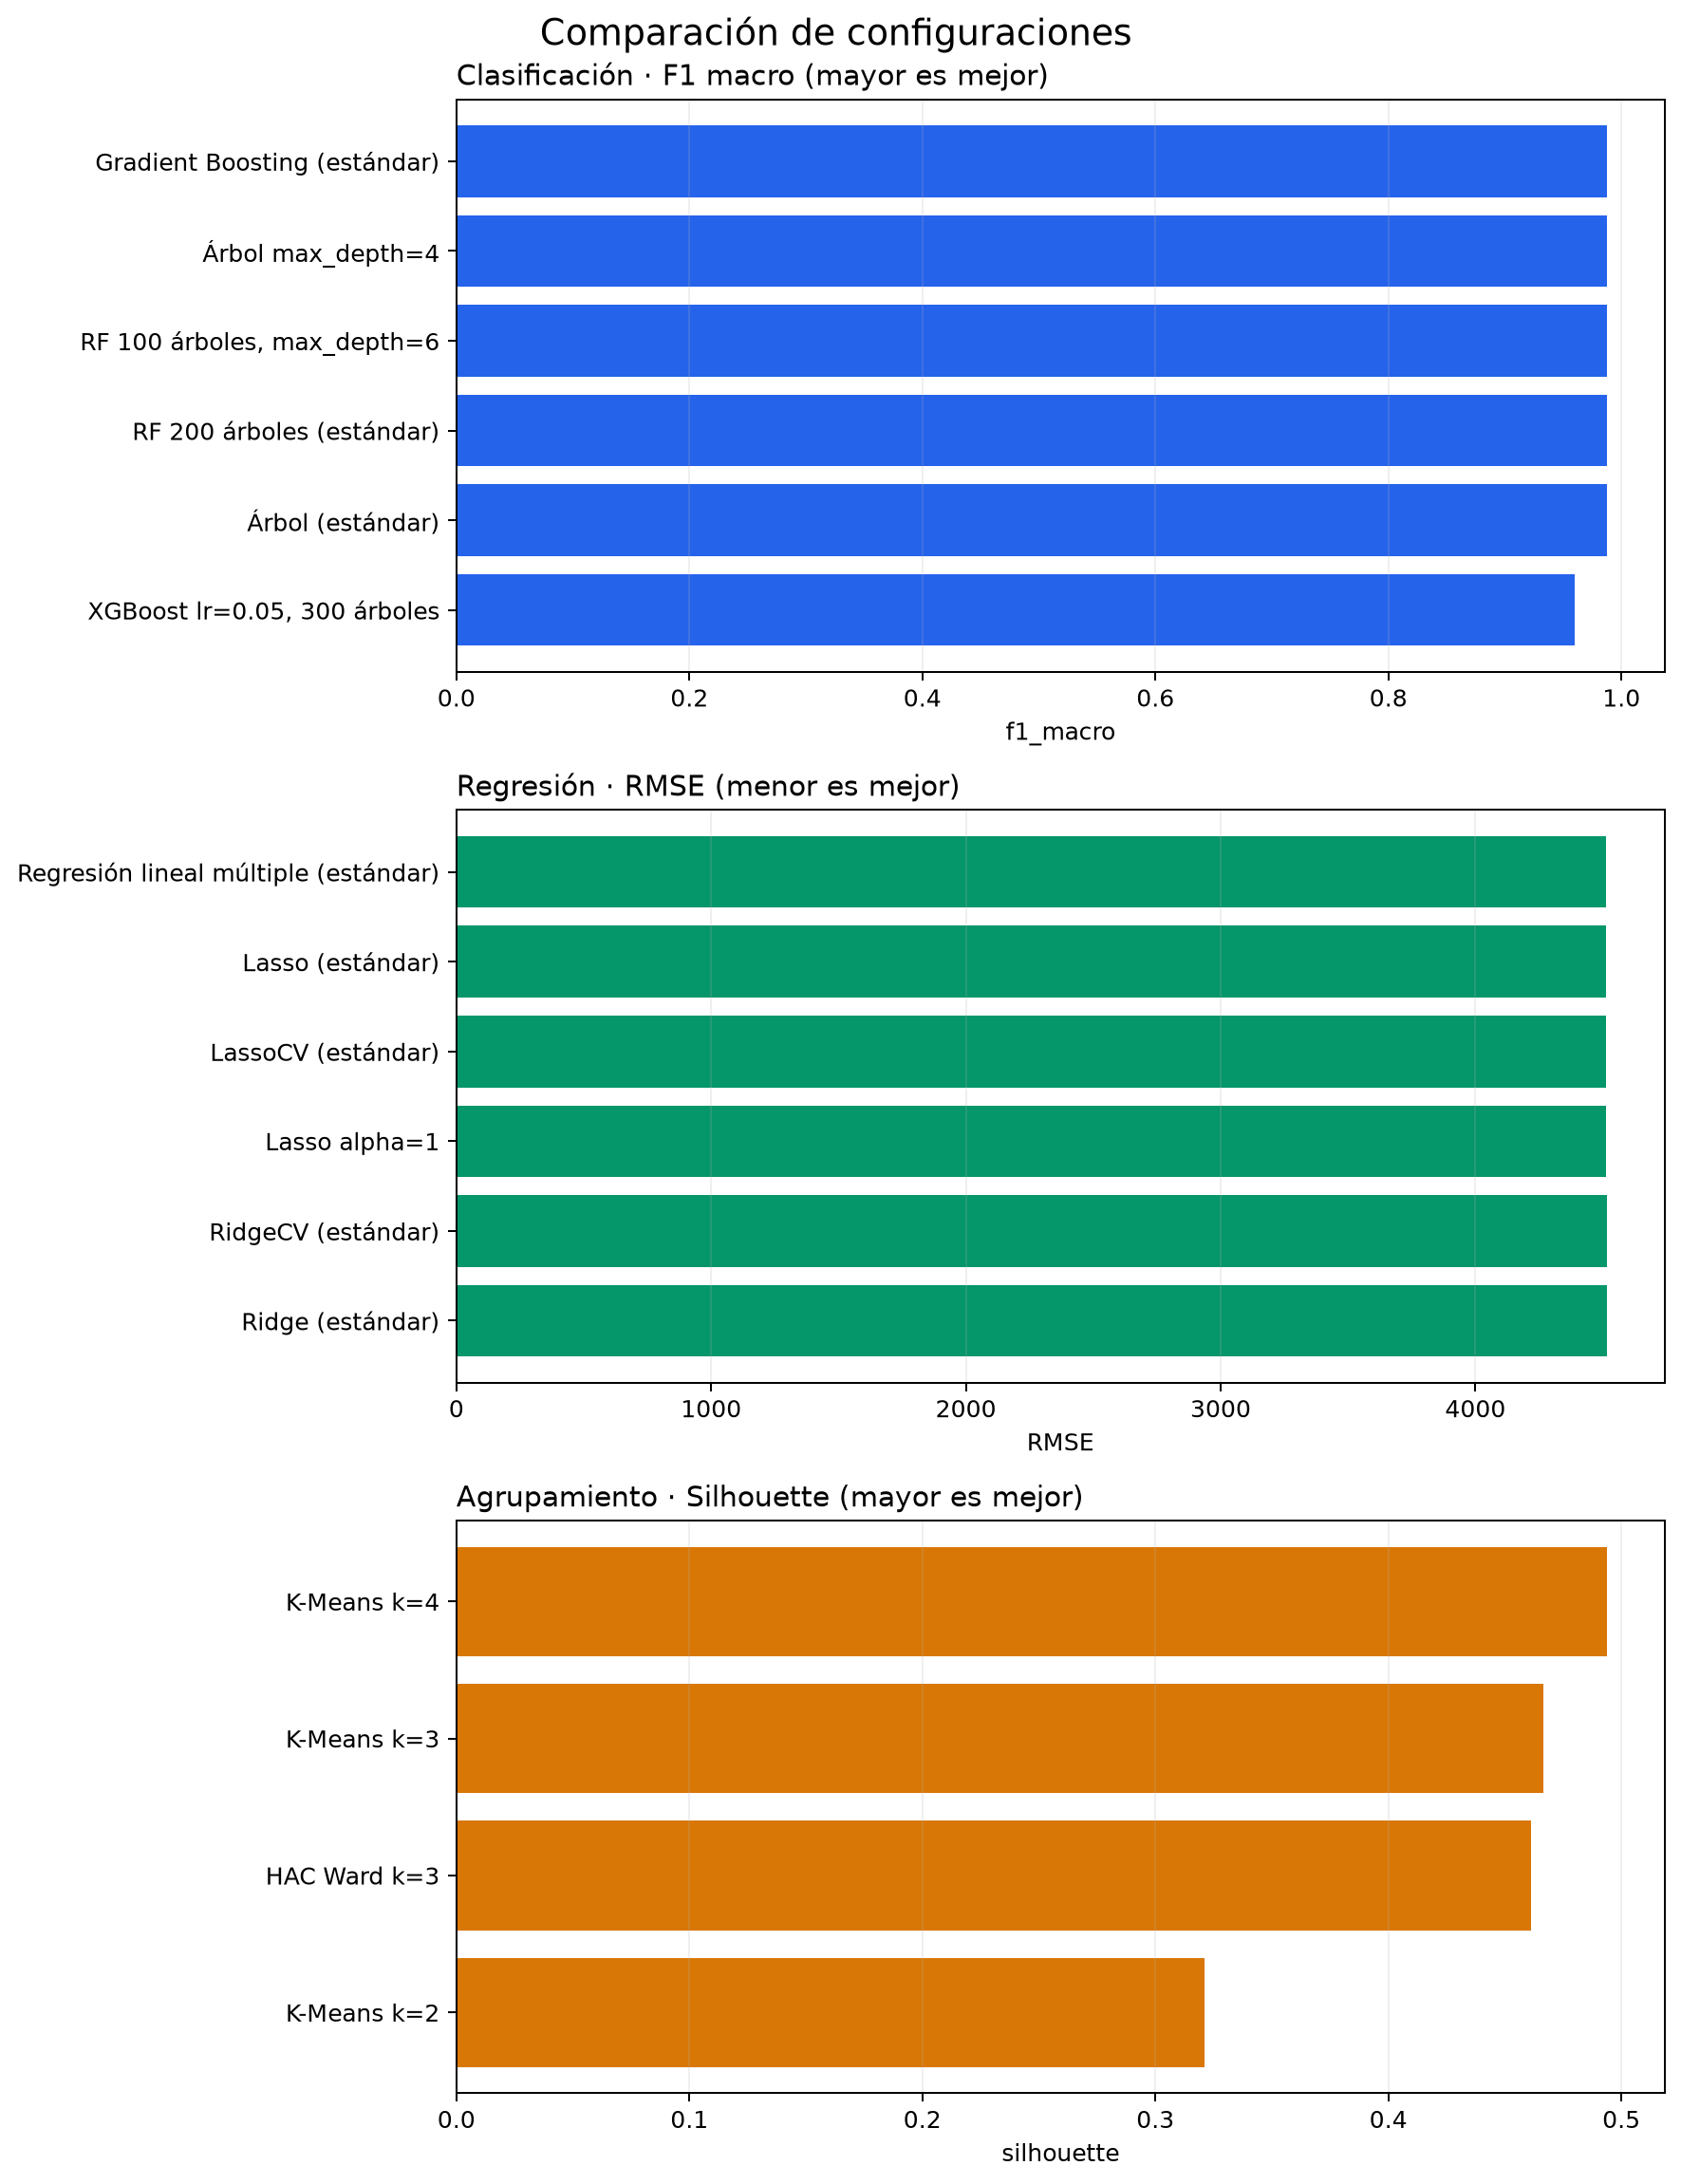
\includegraphics[width=0.88\textwidth]{04_comparacion_benchmarks.png}
  \caption{Comparación de las mejores configuraciones evaluadas en cada tarea. F1 macro y silhouette se maximizan;
  RMSE se minimiza.}
  \label{fig:benchmarks}
\end{figure}

\section{Interpretación y limitaciones}
En \texttt{drug200.csv}, el mejor resultado del benchmark se obtiene con un árbol de decisión; la evaluación
adicional de Random Forest permite revisar la matriz de confusión y el cambio entre tres particiones. En el conjunto
sintético, los modelos lineales obtienen los menores errores entre las configuraciones comparadas, lo cual es
coherente con la construcción aditiva del objetivo. Para la segmentación, K-Means con cuatro grupos alcanza el
mayor silhouette de las configuraciones de agrupamiento evaluadas; la figura usa tres grupos únicamente como una
vista complementaria.

Estos resultados no demuestran generalización a otros datos. Los conjuntos heredados de clasificación y
agrupamiento no incluyen metadatos de procedencia ni licencia en el repositorio; no se atribuye aquí un origen
externo y debe confirmarse antes de redistribuirlos. El conjunto de regresión es sintético. Las métricas dependen
de las columnas, la partición y los parámetros elegidos; no deben interpretarse como evidencia causal ni como
garantía de rendimiento en producción.

\section{Conclusiones}
El proyecto integra en una sola aplicación la carga y preparación de datos, los análisis de aprendizaje automático,
la coordinación multiagente y la presentación de resultados. La separación entre controlador, servicios, backend
ML y agentes permite que las páginas del dashboard soliciten análisis sin instanciar directamente los modelos.
El registro por capacidad, el bus de mensajes y la fábrica ofrecen un mecanismo de extensión y trazabilidad que
se verifica con pruebas automatizadas y una demostración de plugin dinámico.

Los benchmarks reproducibles muestran que el flujo analítico funciona con semillas y configuraciones registradas,
pero no representan una garantía de rendimiento fuera de los conjuntos evaluados. Como trabajo pendiente para una
entrega pública, deben confirmarse las condiciones de uso de los datos heredados y generarse el paquete final con
el nombre requerido por el curso.

\section{Verificación}
La suite automatizada, la cobertura y la demostración de creación dinámica se documentan en
\url{docs/evidencias/README.md}. Las pruebas cubren la mensajería, el registro, el coordinador, el ciclo de vida,
los fallos, la extensión dinámica y la integración del dashboard con el backend. El script de experimentos genera
tablas, figuras y un manifiesto con los conjuntos de entrada, configuraciones, semillas, versión de Python y hashes
SHA-256 en \url{docs/resultados/resultados.json}. Los comandos de generación se describen en el README del
repositorio. Las referencias metodológicas se incluyen a continuación.

\bibliographystyle{plainnat}
\bibliography{references}

\end{document}
